\documentclass{beamer}
\usetheme{Madrid}
 
\usepackage[utf8]{inputenc}

\usepackage{amsmath}
\usepackage{amsfonts}
\usepackage{array}

\usepackage{graphicx}
\graphicspath{{./figs/}}
\usepackage{subcaption}
\captionsetup[subfigure]{labelformat=empty, justification=centering}

\usepackage{multirow}
\usepackage{xspace}


\usepackage{tikz}
\usetikzlibrary{arrows, shapes, positioning}

\usepackage[ruled]{algorithm2e}

%Information to be included in the title page:
\title{Verifiable Random Functions in Blockchains}

\author{Runchao Han}
\institute{}
\date{}

\begin{document}

\frame{\titlepage}

%%%%%%%%%%%%%%%%%%%%%%%%%%%%%%%%%%%%%%%%%%%%%%%%%%%%%%%%%%%%%%%%%%%%%%%%%%%%%%%%%%%%%%%%%%%%%%%%

\begin{frame}
\frametitle{Summary}

\begin{figure}
    \centering
    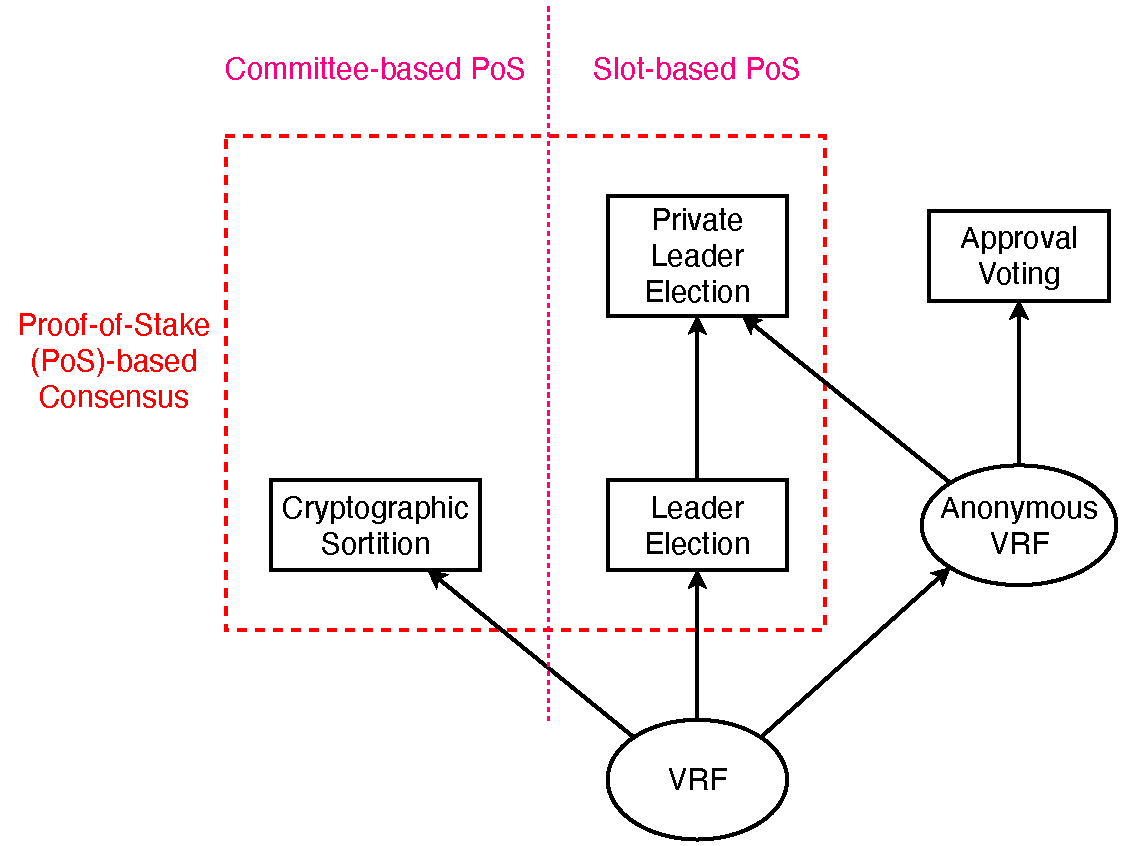
\includegraphics[width=.7\textwidth]{figs/overview.pdf}
\end{figure}

\end{frame}

%%%%%%%%%%%%%%%%%%%%%%%%%%%%%%%%%%%%%%%%%%%%%%%%%%%%%%%%%%%%%%%%%%%%%%%%%%%%%%%%%%%%%%%%%%%%%%%%

\section{Background: Proof-of-Stake-based Consensus}

\begin{frame}
\frametitle{Proof-of-Stake (PoS)-based consensus}

\begin{itemize}
    \item First introduced in PPCoin~\cite{king2012ppcoin}.
    \item First formalised in Ouroboros~\cite{kiayias2017ouroboros}.
    \item Nodes deposit some coins (as \textbf{stake}) to participate in the consensus.
    \item With more stake, the probability that a node can propose blocks will be larger.
\end{itemize}

\begin{figure}
    \centering
    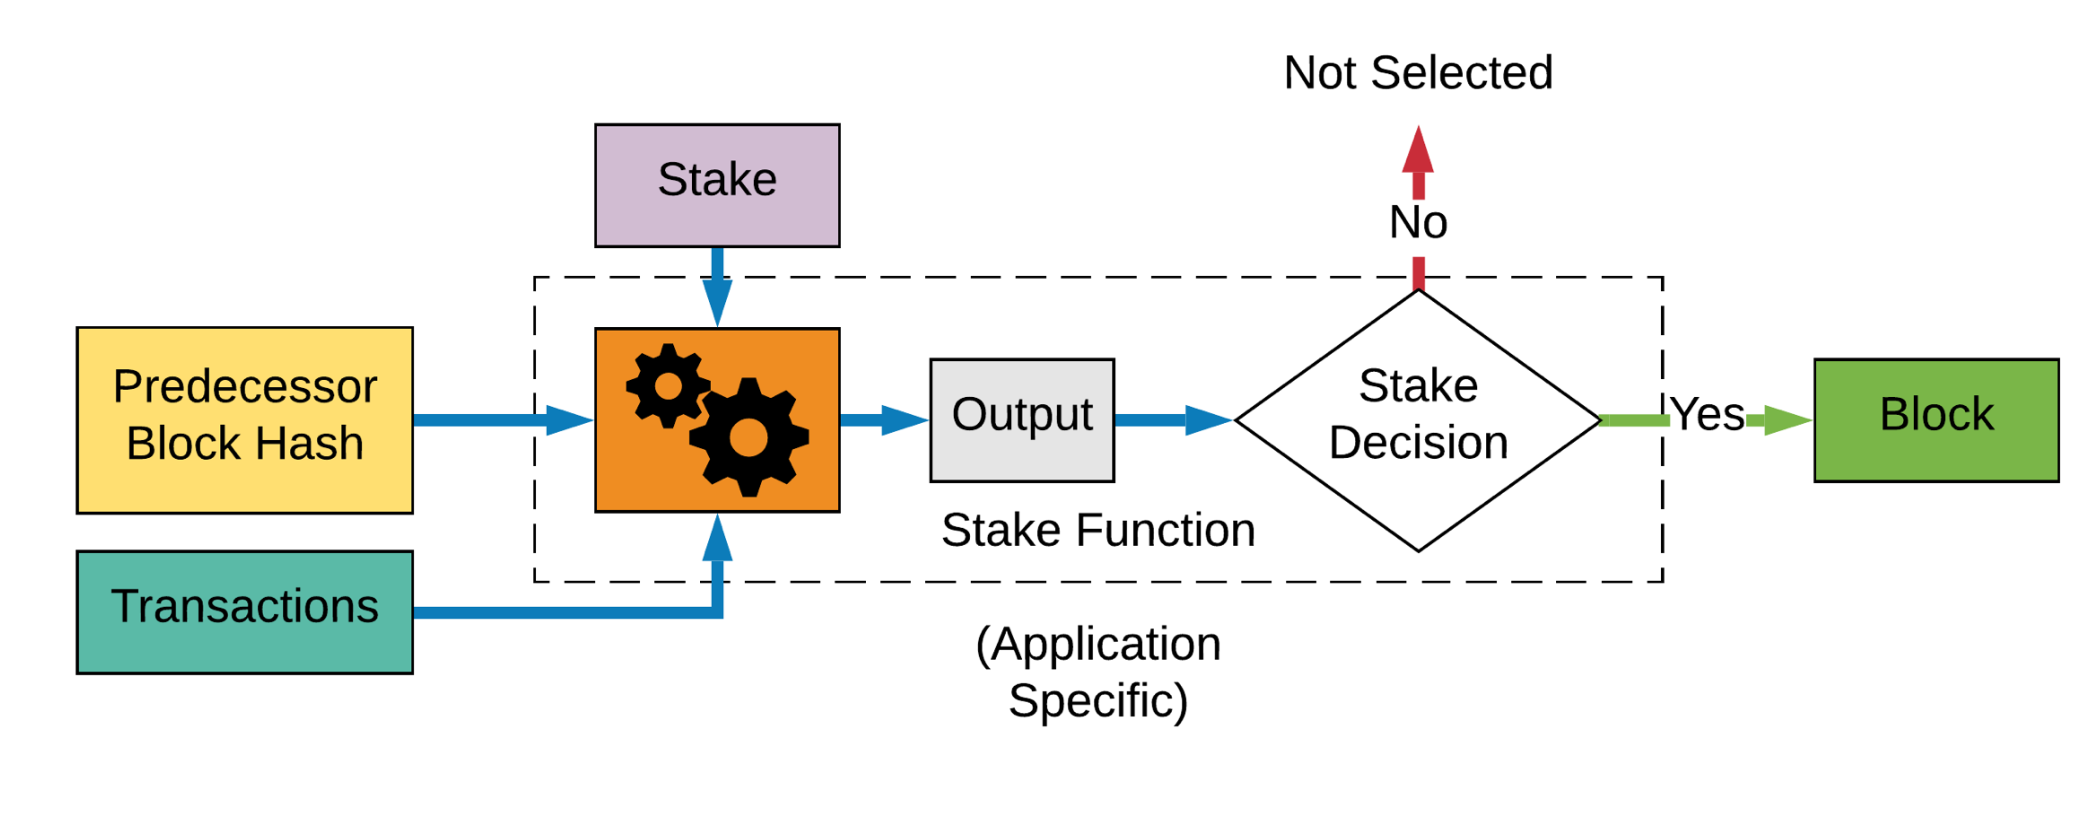
\includegraphics[width=.8\textwidth]{figs/pos-overview.png}
\end{figure}

\end{frame}

\begin{frame}
\frametitle{Two Paradigms of PoS-based Consensus}

Taxonomy from Ganesh et al.~\cite{ganesh2019proof}.

\begin{figure}
    \begin{subfigure}{.45\textwidth}
        \centering
        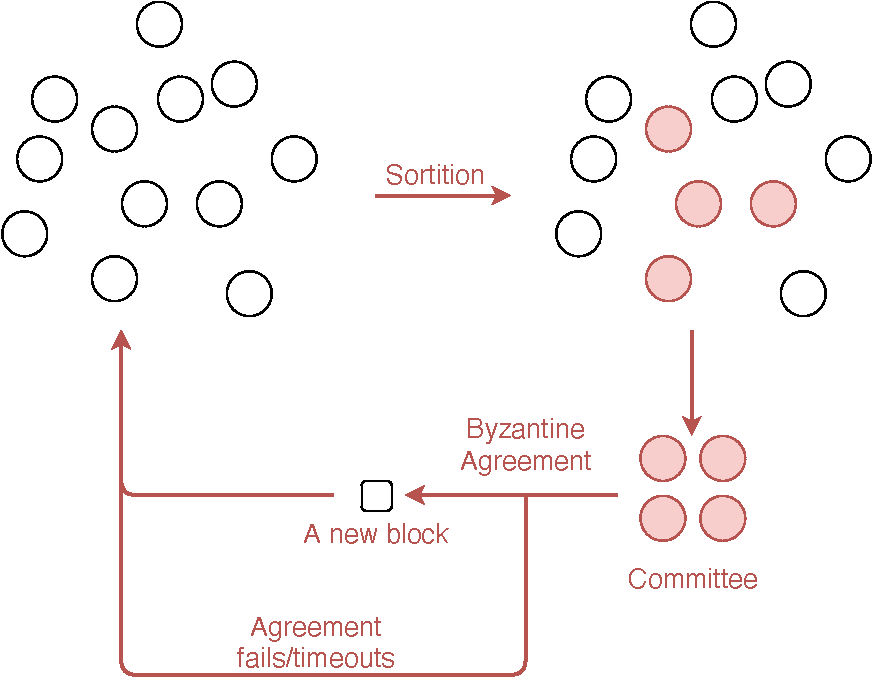
\includegraphics[width=.8\linewidth]{./figs/committee-based-pos.pdf}  
        \caption{Committee-based PoS.\\Employed by Algorand~\cite{gilad2017algorand}.}
    \end{subfigure}
    \hfill
    \begin{subfigure}{.45\textwidth}
      \centering
      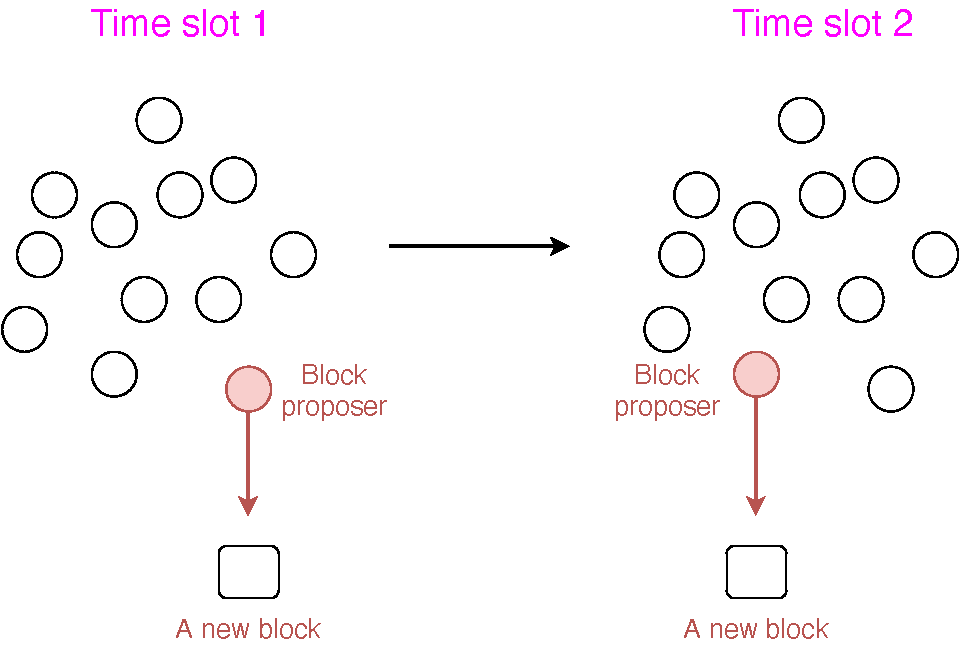
\includegraphics[width=.8\linewidth]{./figs/slot-based-pos.pdf}  
      \caption{Slot-based PoS.\\Employed by the Ouroboros family~\cite{kiayias2017ouroboros, david2018ouroboros, badertscher2018ouroboros, kerber2019ouroboros}.}
    \end{subfigure}
\end{figure}

\end{frame}




\begin{frame}
\frametitle{Key Components using VRFs in PoW-based Consensus}

\begin{figure}
    \begin{subfigure}{.45\textwidth}
        \centering
        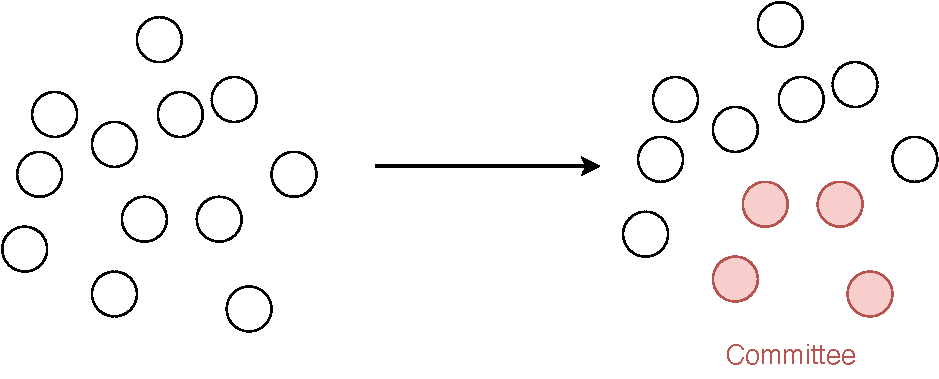
\includegraphics[width=\linewidth]{./figs/sortition.pdf}  
        \caption{Cryptographic Sortition for Committee-based PoS.}
    \end{subfigure}
    \hfill
    \begin{subfigure}{.45\textwidth}
      \centering
      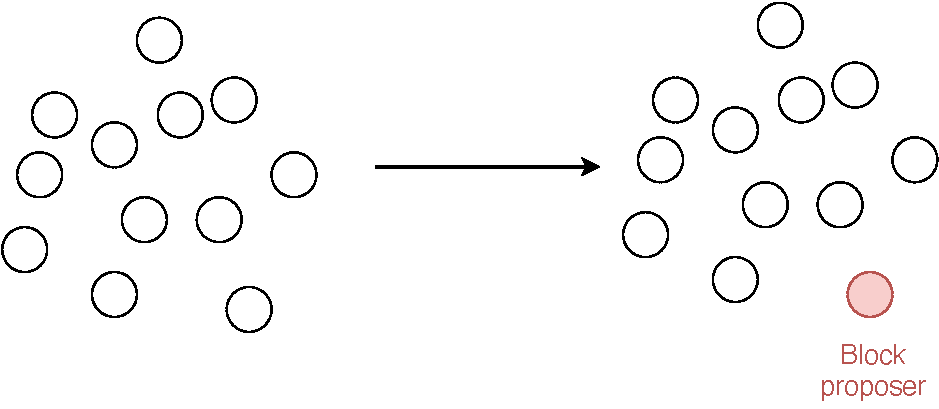
\includegraphics[width=\linewidth]{./figs/leader-election.pdf}  
      \caption{Leader Election for Slot-based PoS.}
    \end{subfigure}
\end{figure}


\end{frame}



%%%%%%%%%%%%%%%%%%%%%%%%%%%%%%%%%%%%%%%%%%%%%%%%%%%%%%%%%%%%%%%%%%%%%%%%%%%%%%%%%%%%%%%%%%%%%%%%


\section{Cryptographic Sortition}


\begin{frame}
\frametitle{Desired Properties of Cryptographic Sortition}

Unfortunately, Cryptographic Sortition has never been formalised...

\begin{itemize}
    \item Only \textbf{a small subset} of users are selected
    \item \textbf{Sybil-resistant}: allocating stakes to multiple users cannot enlarge the chance of being selected
    \item Users are selected \textbf{randomly} while \textbf{weighted by their stakes}.
    \begin{itemize}
        \item More stake, more likely to be selected
        \item Users with little stake still have (very small) chance, rather than no chance
    \end{itemize}
    \item \textbf{Privacy}: an adversary cannot know whether a user is elected before he proves himself
\end{itemize}
    
\end{frame}

\begin{frame}
\frametitle{Basic idea of Algorand's Cryptographic Sortition}

\begin{itemize}
    \item For each user with $w$ coins, divide interval $[0, 1)$ to $w$ sub-intervals $\langle I^j \rangle$.
    \item The user computes a VRF $hash$ of a $seed$, then find $I^j$ s.t. $\frac{hash}{2^{hashlen}} \in I^j$.
    \item More stake, more likely to have a bigger $j$.
    \item Given a cutoff $x$, nodes with $j > x$ will be selected to the committee.
\end{itemize}
    
\end{frame}

\begin{frame}
\frametitle{Details of Algorand's Cryptographic Sortition}

\begin{itemize}
    \item $sk, w$ is the user's secret key and stake.
    \item $\tau$ is a threshold parameter. $W$ is the total supply of coins. $seed$ is a random number.
    \item $B(k; w, p) = {w \choose k} p^k (1-p)^{w-k}$, $\sum_{k=0}^w B(k; w, p) = 1$.
\end{itemize}

\begin{algorithm}[H]
    \DontPrintSemicolon
    $hash, \pi \gets \mathsf{VRF}_{sk}(seed || role)$\;
    $p \gets \frac{\tau}{W}$\;
    $j \gets 0$\;
    \While{$\frac{hash}{2^{hashlen}} \notin \left[ \sum_{k=0}^j B(k;w,p), \sum_{k=0}^{j+1} B(k;w,p) \right)$}{
        $j++$\;
    }
    \Return{$hash,\pi, j$}
    \caption{$\mathsf{Sortition}(sk, seed, \tau, role, w, W)$}
\end{algorithm}

\end{frame}

\begin{frame}
\frametitle{Rationales of Algorand's Cryptographic Sortition}
    
\begin{itemize}
    \item With bigger $\tau$, $j$ is likely to be small.
    \item With bigger $w$, $j$ is likely to be big.
    \item Sybil-resistant by $B(k_1;n_1,p) + B(k_2;n_2,p) = B(k_1 + k_2;n_1 + n_2,p)$.
    \item Acheives Privacy as VRF requires $sk$ to compute.
\end{itemize}

\end{frame}




%%%%%%%%%%%%%%%%%%%%%%%%%%%%%%%%%%%%%%%%%%%%%%%%%%%%%%%%%%%%%%%%%%%%%%%%%%%%%%%%%%%%%%%%%%%%%%%%

\section{Leader Election}



\begin{frame}
\frametitle{Definition of Leader Election}


Recently formalised by Boneh et al.~\cite{bonehsingle} (not stake-based).

\begin{itemize}
    \item \textbf{Uniqueness}: Only one user can prove he is the leader.
    \item \textbf{Unpredictability}: The probability that each honest node is elected is equal.
    \item \textbf{Fairness}: The adversary cannot manipulate the probability distribution in \textbf{Unpredictability}.
\end{itemize}

In stake-based Leader Election, the probability that each node is elected is weighted by his stake.

\end{frame}





\begin{frame}
\frametitle{Ouroboros Praos' Leader Election}

\begin{itemize}
    \item $w, W$ is the user's stake and the total supply of coins, resp.
    \item $f$ is a difficulty parameter. $f \uparrow \Rightarrow P(\text{elected}) \uparrow$.
    \item $sl$ is \# of the time slot.
    \item CANNOT guarantee that only one user is elected.
    \item Sybil-resistant by $1 - \phi_f(\sum_i \alpha_i) = \prod_i(1 - \phi_f(\alpha_i))$.
\end{itemize}

\begin{algorithm}[H]
    \DontPrintSemicolon
    $\alpha \gets \frac{w}{W}$\;
    $p \gets \phi_f(\alpha) = 1 - (1-f)^\alpha$\;
    $T \gets 2^{hashlen} p$\;
    $y, \pi \gets \mathsf{VRF}_{sk}(sl)$\;
    \uIf{$y < T$} {
        \Return{Elected}\;
    }\Else{
        \Return{Not elected}\;
    }
    \caption{Ouroboros Praos' Leader Election}
\end{algorithm}


\end{frame}


\section{Private Proof-of-Stake}

\begin{frame}
\frametitle{Private Proof-of-Stake (PPoS)}

\begin{itemize}
    \item Existing approaches require elected users to reveal their identities/wealth.
    \item To construct PoS-based privacy-preserving cryptocurrencies, these info should be hidden.
    \item This comes to the research problem of Private Proof-of-Stake (PPoS):
\end{itemize}

\centerline{\color{red} Is it possible for them to hide identities and wealth in PoS?}

\begin{itemize}
    \item PPoS is introduced in two concurrent papers: Ouroboros Crypsinous~\cite{kerber2019ouroboros} and Ganesh et al.~\cite{ganesh2019proof}.
    \item Ganesh et al.~\cite{ganesh2019proof} construct PPoS from Anonymous Verifiable Random Functions (AVRF).
\end{itemize}

\end{frame}


\begin{frame}
\frametitle{Anonymous Verifiable Random Functions (AVRF)}
    
\begin{itemize}
    \item The verification should not reveal the public key.
    \item A secret key is associated with many public keys.
    \item Two VRF hashes on the same secret key but different messages cannot be linked to a public key.
\end{itemize}

\begin{figure}
    \centering
    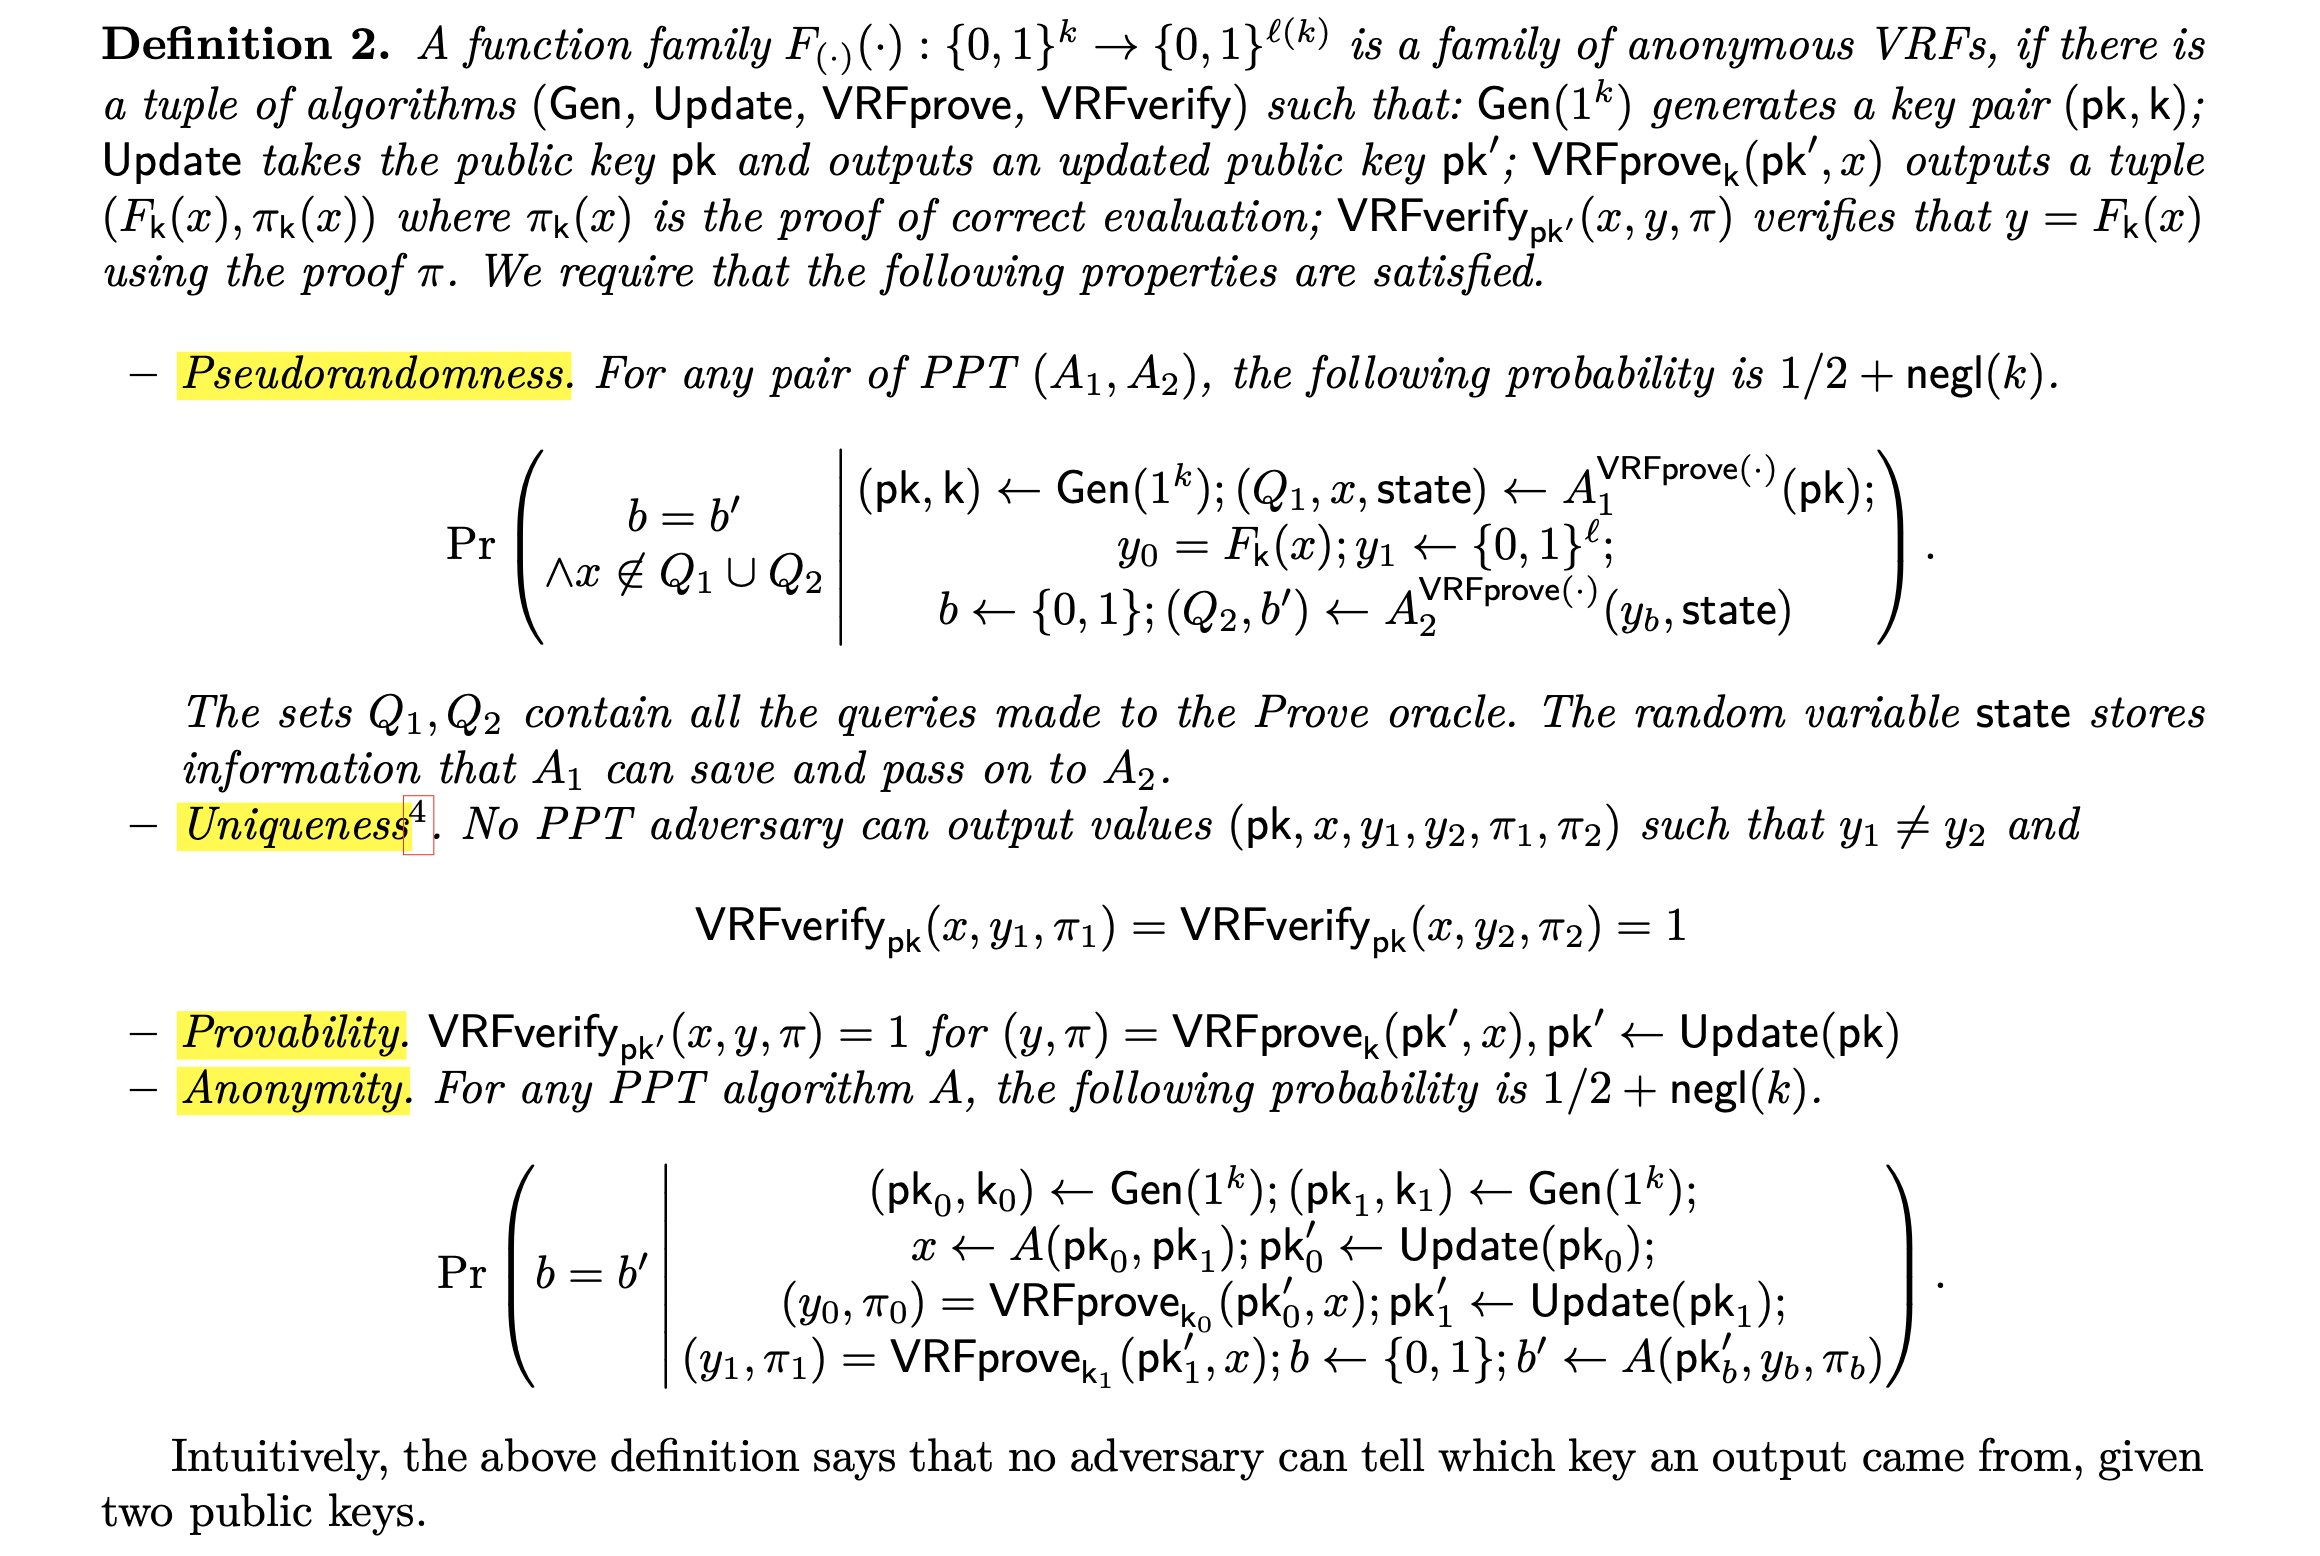
\includegraphics[width=.7\textwidth]{figs/avrf-def.png}
\end{figure}


\end{frame}


\begin{frame}
\frametitle{An AVRF Construction}

\begin{description}
    \item[$\mathsf{Gen}(1^k) \to (pk, k)$]: Choose a generator $g$ of $G$; choose a random secret key $k \stackrel{\$}{\gets} \mathbb{Z}_q$; output $pk = (g, g^k)$, $k$.
    \item[$\mathsf{Update}(pk) \to pk'$]: Let $pk$ be $g, v$; choose a random $r \stackrel{\$}{\gets} \mathbb{Z}_q$; $g' = g^r$, $v' = v^r$; output $pk' = (g', v')$.
    \item[$\mathsf{VRFprove}_k(pk', x) \to (pk', y, \pi)$]: Let $pk'$ be $g, v$; $u = H(x), y = u^k$; $\pi' = NIZK: \{k: log_uy = log_gv\}$; $pi = (u, \pi')$; output $pk', y, \pi$.
    \item[$\mathsf{VRFVerify}_{pk'}(x, y, \pi) \to \{0, 1\}$]: Output 1 if $u = H(x)$ and $\pi$ verifies; otherwise 0.
\end{description}

\end{frame}


\begin{frame}
\frametitle{Private Ouroboros Praos from AVRF}

\begin{itemize}
    \item $w$ and $W$ are represented as $s$ bits.
    \item $w$ is represented as $s$ bits $\langle b_i \rangle$. $\sum_{i=0}^{s-1} 2^i b_i$.
    \item As long as one bit satisfies $y_i < T_i$, the user is elected.
\end{itemize}

\begin{algorithm}[H]
    \DontPrintSemicolon
    \For{$i \in [0, s-1]$}{
        $pk_i \stackrel{\$}{\gets} \mathsf{Update}(pk)$\;
        $\alpha_i \gets \frac{2^i b_i}{W}$\;
        $p_i \gets \phi_f(\alpha_i) = 1 - (1-f)^{\alpha_i}$\;
        $T_i \gets 2^{hashlen} p_i$\;
        $y_i, \pi_i \gets \mathsf{VRFprove}_k(pk_i, i || sl)$\;
        \uIf{$y_i < T_i$} {
            Elected\;
        }
    }
    Not elected\;
    \caption{Private Ouroboros Praos. The user has key pair $(k, pk)$.}
\end{algorithm}

\end{frame}




\section{Approval Voting from AVRF}

\begin{frame}
\frametitle{Approval Voting from AVRF}

Approval Voting:
\begin{itemize}
    \item A group of users can vote any number of candidates.
    \item The winner is the candidate with most votes.
    \item Voters should be anonymous.
    \item Each voter can only vote each candidate no more than once.
\end{itemize}

Construction:
\begin{itemize}
    \item Each user $i$ registers an AVRF public key $pk_i$.
    \item To vote a candidate $x$, user $i$ 1) publishes $pk_i' = \mathsf{Update}(pk_i)$, and 2) publishes $(y, \pi) = \mathsf{VRFprove}_{k_i}(pk_i', x)$.
    \item Upon a pair of $(y, \pi)$: If 1) $y$ has appeared, 2) $y$ can be linked to another vote, or 3) $\pi$ does not verify, discard this vote. Otherwise, accept this vote.
\end{itemize}

\end{frame}

\begin{frame}[allowframebreaks]
    \frametitle{References}
    \bibliographystyle{alpha}
    \tiny\bibliography{refs}
\end{frame}

\end{document}